\input{header}

\AtBeginSubsection[]
{
	\begin{frame}<beamer>
		\frametitle{Outline}
		\tableofcontents[current,currentsubsection]
	\end{frame}
}

\begin{document}

\begin{frame}[allowframebreaks] \frametitle{Nondeterministic TM}
  \begin{itemize}
\item $\delta$:
  \begin{equation*}
    \delta: Q\times \Gamma
\rightarrow P(Q\times \Gamma \times \{L,R\})
  \end{equation*}
$P$: power set

\item Example:
  \begin{eqnarray*}
    q_0,a & \rightarrow & q_1,b,R\\
& \rightarrow & q_2, c, L
  \end{eqnarray*}
\item What if 
  \begin{eqnarray*}
    q_0,a & \rightarrow & q_{accept} \\
& \rightarrow & q_{reject}
  \end{eqnarray*}

\item
  For NTM, $w$ accepted if one branch works

\item
  In this sense, unless all branches are finite

\item
  NTM $\rightarrow$ accept or endless loop

\item
  NTM: like an ``acceptor''

\end{itemize}\end{frame} \begin{frame}[allowframebreaks] \frametitle{Example of NTM}
  \begin{itemize}
\item 
$A = \{w\mid w\mbox{ contains } aab\}$
\item State diagram

  \begin{center}
    \begin{tikzpicture}
  \node[state,initial] (q_0) {$q_0$};
  \node[state,right of=q_0] (q_1) {$q_1$};
  \node[state,right of=q_1] (q_2) {$q_2$};
  \node[state,right of=q_2] (q_a) {$q_a$};
  \node[state,below right of=q_0,yshift=-0.5cm] (q_r) {$q_r$};
  \path (q_0) edge[loop above] node{
      $a, b \rightarrow a, b,$ R
    } (q_0);
  \path (q_0) edge[above] node{
      $a \rightarrow$ R
  } (q_1);
  \path (q_1) edge[above] node{
      $a \rightarrow$ R
  } (q_2);
  \path (q_2) edge[above] node{
      $b \rightarrow$ R
    } (q_a);
  \path (q_0) edge[left] node{
      $\sqcup \rightarrow$ R      
    } (q_r);
  \path (q_1) edge[right] node{
    \begin{tabular}{l}
      $b \rightarrow$ R\\
      $\sqcup \rightarrow$ R      
    \end{tabular}
    } (q_r);
  \path (q_2) edge[right, bend left] node{
    \begin{tabular}{l}
      $a \rightarrow$ R\\
      $\sqcup \rightarrow$ R      
    \end{tabular}
    } (q_r);
    \end{tikzpicture}
  \end{center}
%   \begin{center}
%     \begin{pspicture}(-.2,-.5)(9,4)% \showgrid
%       \psset{radius=.3}
% \rput(.5,2.5){\circlenode{0}{$q_0$}}
% \rput(2.5,2.5){\circlenode{1}{$q_1$}}
% \rput(4.5,2.5){\circlenode{2}{$q_2$}}
% \rput(2.5,0.0){\circlenode{3}{$q_r$}}
% \rput(6.5,2.5){\circlenode{4}{$q_a$}}
% \ncline{->}{0}{1}
% \ncline{->}{1}{2}
% \ncline{->}{2}{4}
% \ncline{->}{0}{3}
% \ncline{->}{1}{3}
% \ncline{->}{2}{3}
% \pnode(-.2,2.5){B}
% \ncline{->}{B}{0}
% \rput(1.4,2.7){$a \rightarrow R$}
% \rput(3.4,2.7){$a \rightarrow R$}
% \rput(5.4,2.7){$b \rightarrow R$}
% \rput(0.6,1.5){$\sqcup \rightarrow R$}
% \rput(3.1,1.5){$\sqcup \rightarrow R$}
% \rput(3.1,1.8){$b \rightarrow R$}
% \rput(4.5,1.5){$\sqcup \rightarrow R$}
% \rput(4.5,1.8){$a \rightarrow R$}
% \nccircle{<-}{0}{.4}
% \rput(0.5,3.6){$a,b\rightarrow a,b,R$}
%     \end{pspicture}
%   \end{center}

  
\item You may recall that this is an NFA example discussed before
  
\item Only the first node is nondeterministic

\end{itemize}\end{frame} \begin{frame}[allowframebreaks] \frametitle{Example of NTM}
  \begin{itemize}
\item $L=\{0^n\mid n \mbox{ composite number}\}$
\item From p. 204 of Lewis and Papadimitriou
\item Composite number: product of two natural numbers
\item Procedure
  \begin{itemize}
  \item Nondeterministically choose $p$ and $q$

  \item [] Sequentially try $p$ from $1$ to $n$

  \item Check if $n=pq$

  \item [] This can be done by the earlier example
    \begin{equation*}
    \{a^n b^p c^q\mid n = p \times q\}
  \end{equation*}
  \end{itemize}
\item Question: details about ``non-deterministically'' choose $p$ and $q$?
\item If we sequentially try all $(p,q)$ combinations, then
  looks like we have a deterministic setting?
  
\item Our generation of  $p$ and $q$ can be non-deterministic
\item Say we do a copy operation to generate $p$ elements. The TM can
  have an $\epsilon$ link to stop at any time point
\end{itemize}\end{frame} \begin{frame}[allowframebreaks] \frametitle{Nondeterministic TM $
\equiv$ deterministic TM}
  \begin{itemize}
\item 
$\Leftarrow$ easy
\item
  [] A deterministic TM is a nondeterministic TM

\item
  $\Rightarrow$ more difficult
\item
  Like NFA we use a tree for processing the input
(\# branches finite)
\item
  To traverse a tree we can do
  \begin{center}
  depth-first search
\end{center}
  or
  \begin{center}
  breadth-first
\end{center}
\item If using depth-first search, one branch 
may lead to $\infty$ steps
\item [] Then we cannot consider other branches even if the
  input is accepted

  
\item
  Thus we should consider breadth-first
  
\item Fig 3.17: a deterministic TM to simulate a nondeterministic TM

\begin{center}
  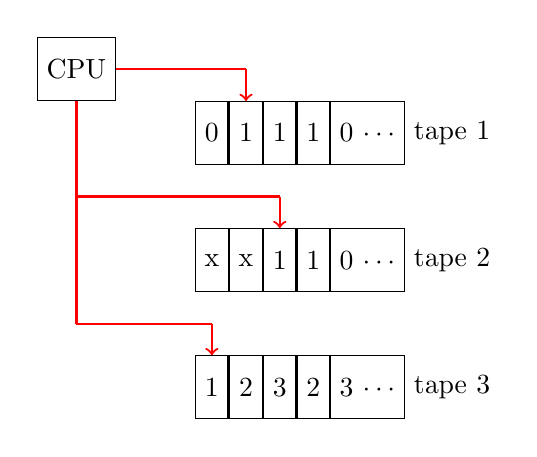
\begin{tikzpicture}[ampersand replacement=\&]
\matrix[nodes={minimum height=8mm}]     
{
  \node[draw](0) {CPU}; \& [1cm]  \& \node(1){} ; \&\&\& \& \\
  \& \node[draw]{0}; \& \node[draw](a){1}; \& \node[draw]{1}; \& \node[draw]{1};  \& \node[draw]{0 $\cdots$};  \& \node{tape 1};\\
\node(2){} ; \&  \&  \& \node(21){} ; \&\& \&\\  
\& \node[draw]{x}; \& \node[draw]{x}; \& \node[draw](b){1}; \& \node[draw]{1}; \& \node[draw]{0 $\cdots$}; \& \node{tape 2};  \\
\node(3){} ; \& \node(31){} ; \&  \&\& \& \&\\
\& \node[draw](c){1}; \& \node[draw]{2}; \& \node[draw]{3}; \& \node[draw]{2}; \& \node[draw]{3 $\cdots$}; \&  \node{tape 3}; \\
};

\draw [-,red,thick] (0) -- (1.center) ;
\draw [->,red,thick] (1.center) -- (a) ;
\draw [-,red,thick] (0) -- (2.center) ;
\draw [-,red,thick] (2.center) -- (21.center) ;
\draw [->,red,thick] (21.center) -- (b) ;
\draw [-,red,thick] (0) -- (3.center) ;
\draw [-,red,thick] (3.center) -- (31.center) ;
\draw [->,red,thick] (31.center) -- (c) ;
\end{tikzpicture}
\end{center}
  
\item 
Tape 1: input, never altered

\item
  Tape 2: process one branch

\item
  Tape 3: maintain the tree

\item
  The key is the 3rd tape

\item
  Suppose $\max$ \# branches 3

\item
  [] At the 1st step: if contents of 3rd tape are 1 2 
\item
  [] $\Rightarrow $ can go to
1 or 2 from $q_0$

\item The tree keeps growing. For example, 

  \begin{alltt}
    1 2
    12 13 2
    12 13 21 22 23
    121 123 13 21 22 23
  \end{alltt}
\item What if 12 is a failed branch?

  \begin{alltt}
    \alert{12} 13 21 22 23
    \alert{12} 131 132 21 22 23
  \end{alltt}

\item
  12 fails, continue 131, no need to remove 12

\end{itemize}\end{frame}

% \begin{frame}[allowframebreaks] \frametitle{Corollary 3.18}
%   \begin{itemize}
% \item omit

% \end{itemize}\end{frame}

\begin{frame}[allowframebreaks] \frametitle{Corollary 3.19}
  \begin{itemize}
\item Definition: NTM is a decider if all branches halt on all inputs


\item Language decidable $\Leftrightarrow$
some NTM decides it

\item
  $\Rightarrow$ easy, one TM decides it and TM is an NTM

\item
  [] This TM halts on all inputs (one branch)

\item
  $\Leftarrow$:
\item
  [] Now NTM terminates on all branches 

\item
  [] We will construct a TM to accept the language
\begin{itemize}
\item each branch is finite

\item [] every input halts $\exists $ a finite max length
\item \# branches finite at each node

\item
  [] The tree to process this input is finite
\item Write it in the 3rd tape
\item We know a multi-tape TM is equivalent to a single-tape TM
\end{itemize}

\end{itemize}\end{frame}

% \begin{frame}[allowframebreaks] \frametitle{Enumerators}
%   \begin{itemize}
% \item the description from the book is rather
% unclear

% We will discuss only basic concepts

% Show figure in the book


% \item $L=0\{0,1\}^*$, the printer

% 0\\
% 00\\
% 01\\
% 000\\
% 001

% Basically all accepted sequences


% \item Printer is like another tape

% 0\#00\#01\#000...
% \end{itemize}\end{frame} \begin{frame}[allowframebreaks] \frametitle{How enumerator simulates a TM}
%   \begin{itemize}
%   \item
%     head never moves left
% \item Consider $\Sigma^*$ as 

% 0,1,00,01,10,11,...
% \item call them $s_1,s_2,\ldots$
% \item Enumerator:

% repeat $i=1,2,\ldots$

% run TM with $i$ steps on $s_1, \ldots, s_i$

% if any $s_j$ accepts, print it

% \item Any given $s$ recognized by TM will 

% be accepted by the enumerator at one point
% \end{itemize}\end{frame}



\end{document}

%%% Local Variables:
%%% mode: latex
%%% TeX-master: t
%%% End:

